
\section{Validazione}
 

\subsection{Scelte progetturali}

\subsection{Strumenti automatici}
Per garantire che il sito sia correttamente visualizzato e che rimanga accessibile nel maggior numero di browser possibili si è verificata la validità di tutte le pagine tramite l'utilizzo di molteplici validator e sono stati effettuati dei test di visualizzazione su browser meno recenti.


\subsubsection{Audits}
Audits è uno strumento automatizzato open-source per migliorare la qualità delle pagine web.
I punteggi del report di Audits rappresentano il punteggio della pagina per quella particolare categoria.
\begin{figure}[H]
	\centerline{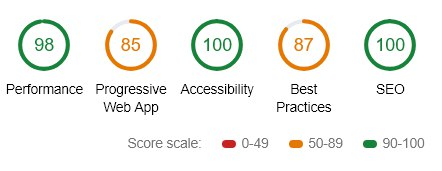
\includegraphics[scale= 0.33]{img/punteggiAudits.png}}
	\caption{Punteggi restituiti per ogni categoria}
\end{figure}



\subsubsection{Markup Validation Service w3.org}
Tutte le pagine dell'utente generico sono state validate attraverso questo validatore. 

\subsubsection{W3C CSS Validator w3.org}
Tutti i fogli di stile sono stati validati con questo validatore e non hanno riportato errori o warnings.

\subsubsection{TotalValidator}
Tutte le pagine sono state validate utilizzando Total Validator, e non hanno riportato errori o warnings.


\subsection{Test effettuati}
Il sito è stato testato con successo su: Google Chrome, Mozilla Firefox e Internet Explorer. Nessuno di questi browser ha dato problemi riguardanti l'utilizzo e le funzionalità della piattaforma.
\\Inoltre sono stati effettuati dei test anche per la versione mobile, in particolare su:
\begin{itemize}
	\item Huawei Honor 9;
	\item Iphone 6; 
	\item Motorola g6 plus;
\end{itemize}
L’usabilità del sito web rimane invariata per ogni dispostivo essendo stato sviluppato in modo da essere responsive.
